\setlinespacing{1.1}

\chapter{Data Acquisition} \label{sec:Data_Acquisition}

\section{section header 1}

\subsection{Subsection header 1}
fdsdfsdfds
\subsection{Subsection header 2}
fdsdfsdfds
\subsection{Subsection header 3}
fdsdfsdfds

\section{section header 2}

\subsection{Subsection header 1}

Figure \ref{Figure: Map of the Greater Dublin Area} shows a spatial map of the
GDA.

\begin{figure}[htbp]
    \center 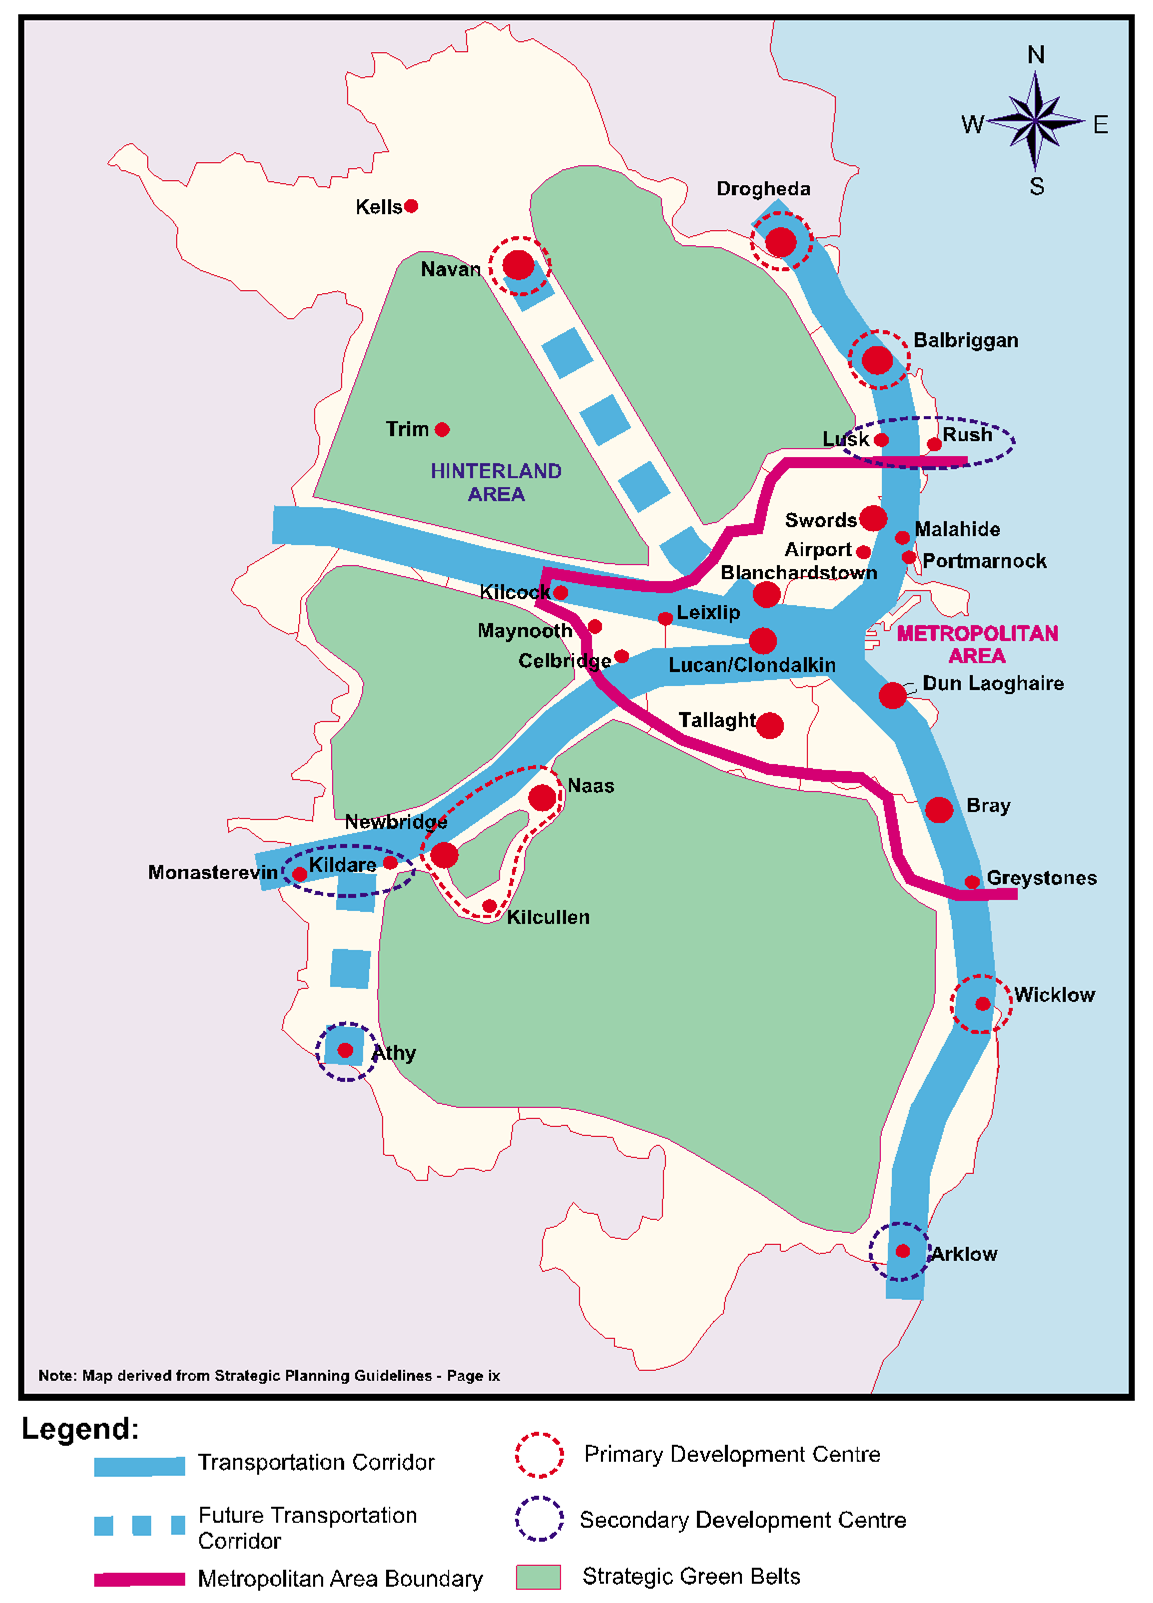
\includegraphics[width=400pt]{./image/intro1}\\
    \caption{Map of the Greater Dublin Area \citep{PLA01}} \label{Figure: Map of the Greater Dublin
        Area}
\end{figure}

\newpage

\begin{table}[htbp]
    \footnotesize{} \setlinespacing{1.0} \vspace{10pt} \begin{longtable} {p{190pt}cccc}
        \caption{Demographic Projections of the GDA}                                 \\
        \hline

        \textbf{Greater Dublin Area} &

        \textbf{1991}                & \textbf{1996} & \textbf{1999} & \textbf{2016} \\* \hline \hline {Population
        (million) }                  &

        {1.35}                       & {1.41}        & {1.46}        & {1.75}        \\* \hline {Households ('000) } &

        {402}                        & {446}         & {521}         & {675}         \\* \hline {Employment ('000) } &

        {452}                        & {549}         & {681}         & {878}         \\* \hline {Unemployment rate } &

        {16{\%}}                     & {12{\%}}      & {6{\%}}       & {5{\%}}       \\* \hline {Car Ownership (per 1000 population)} &

        {247}                        & {292}         & {342}         & {480}         \\* \hline {{\%} Growth in GDP since 1991} & {- } & {42{\%}} & {79{\%}} &
        {260{\%} }                                                                   \\* \hline

        \label{Table: Demographic Projections of the GDA}
    \end{longtable}
    \normalsize{} \setlinespacing{1.1}
\end{table}

\newpage

\begin{figure}[htbp]
    \center 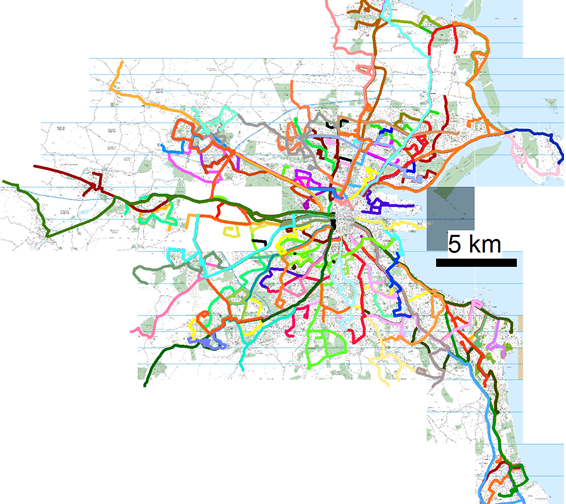
\includegraphics[width=400pt]{./image/intro2}\\
    \caption{Map of Bus Routes of Dublin Bus} \label{fig2: Map of bus routes provided by Dublin Bus}
\end{figure}

The figures shown in Table \ref{Table: Demographic Projections of the GDA} are
taken from the website of Dublin Bus \citep{DUB05}. The bus fleet is broken
down into depot location and bus category.

\subsection{Subsection header 2}
fdsdfsdfds
\subsection{Subsection header 3}
fdsdfsdfds

\section{section header 3}

\subsection{Subsection header 1}
fdsdfsdfds
\subsection{Subsection header 2}
fdsdfsdfds
\subsection{Subsection header 3}
fdsdfsdfds

\section{section header 4}

\subsection{Subsection header 1}

Latex is very good when mathematical formulas need to be displayed:

\begin{equation}\label{taeq2}
    S_{ij}=1-{\frac{|(F_{ij}-F^T_{ij})|}{(F_{ij}+F^T_{ij})}}
\end{equation}

\subsection{Subsection header 2}
\subsection{Subsection header 3}
